%
% Niniejszy plik stanowi przykład formatowania pracy magisterskiej na
% Wydziale MIM UW.  Szkielet użytych poleceń można wykorzystywać do
% woli, np. formatujac wlasna prace.
%
% Zawartosc merytoryczna stanowi oryginalnosiagniecie
% naukowosciowe Marcina Wolinskiego.  Wszelkie prawa zastrzeżone.
%
% Copyright (c) 2001 by Marcin Woliński <M.Wolinski@gust.org.pl>
% Poprawki spowodowane zmianami przepisów - Marcin Szczuka, 1.10.2004
% Poprawki spowodowane zmianami przepisow i ujednolicenie 
% - Seweryn Karłowicz, 05.05.2006
% Dodanie wielu autorów i tłumaczenia na angielski - Kuba Pochrybniak, 29.11.2016

% dodaj opcję [licencjacka] dla pracy licencjackiej
% dodaj opcję [en] dla wersji angielskiej (mogą być obie: [licencjacka,en])
\documentclass[licencjacka]{pracamgr}
\usepackage{amsmath}
\usepackage{graphicx}

% Dane magistranta:
\autor{Tomasz Fąs}{382348}


% Dane magistrantów:
%\autor{Autor Zerowy}{342007}
%\autori{Autor Pierwszy}{342013}
%\autorii{Drugi Autor-Z-Rzędu}{231023}
%\autoriii{Trzeci z Autorów}{777321}
%\autoriv{Autor nr Cztery}{432145}
%\autorv{Autor nr Pięć}{342011}

\title{Tunelowanie między studniami kwantowymi umieszczonymi w mikrownęce optycznej.}


%\tytulang{An implementation of a difference blabalizer based on the theory of $\sigma$ -- $\rho$ phetors}

%kierunek: 
% - matematyka, informacyka, ...
% - Mathematics, Computer Science, ...
\kierunek{Fizyka}

% informatyka - nie okreslamy zakresu (opcja zakomentowana)
% matematyka - zakres moze pozostac nieokreslony,
% a jesli ma byc okreslony dla pracy mgr,
% to przyjmuje jedna z wartosci:
% {metod matematycznych w finansach}
% {metod matematycznych w ubezpieczeniach}
% {matematyki stosowanej}
% {nauczania matematyki}
% Dla pracy licencjackiej mamy natomiast
% mozliwosc wpisania takiej wartosci zakresu:
% {Jednoczesnych Studiow Ekonomiczno--Matematycznych}

% \zakres{Tu wpisac, jesli trzeba, jedna z opcji podanych wyzej}

% Praca wykonana pod kierunkiem:
% (podać tytuł/stopień imię i nazwisko opiekuna
% Instytut
% ew. Wydział ew. Uczelnia (jeżeli nie MIM UW))
\opiekun{dr hab. Jan Suffczyński\\
  Zakład Fizyki Ciała Stałego\\
  }

% miesiąc i~rok:
\date{Któryś z 2019}

%Podać dziedzinę wg klasyfikacji Socrates-Erasmus:
\dziedzina{ 
%11.0 Matematyka, Informatyka:\\ 
%11.1 Matematyka\\ 
13.2 Fizyka\\ 
%11.3 Informatyka\\ 
%11.4 Sztuczna inteligencja\\ 
%11.5 Nauki aktuarialne\\
%11.9 Inne nauki matematyczne i informatyczne
}

%Klasyfikacja tematyczna wedlug AMS (matematyka) lub ACM (informatyka)
\klasyfikacja{Do\\
  ustalenia\\
  chyba}

% Słowa kluczowe:
\keywords{mikrownęka optyczna, tunelowanie, polaryton, ekscyton, fotoluminescencja}

% Tu jest dobre miejsce na Twoje własne makra i~środowiska:
\newtheorem{defi}{Definicja}[section]

% koniec definicji

\begin{document}

\maketitle

%tu idzie streszczenie na strone poczatkowa
\begin{abstract}
  W niniejszej pracy przedstawiono zależność intensywności tunelowania między studniami kwantowymi od przyłożonego pola magnetycznego. Wykorzystana próbka składała się ze studni kwantowych umieszczonych w mikrownęce. Udało się uzyskać tunelowanie całego ekscytonu tj. elektronu i dziury, przez barierę potencjału o szerokości 125 nm. Doświadczenie to częściowo wypełnia lukę w dziedzinie tunelowania średniodystansowego.
\end{abstract}

\tableofcontents
%\listoffigures
%\listoftables

\chapter*{Wprowadzenie}
\addcontentsline{toc}{chapter}{Wprowadzenie}
%Miesznie funkcji falowych%
%Ogólny opis, bez wzgłębiania się w szcegóły
%
Jednym z ważniejszych efektów w mechanice kwantowej jest tunelowanie, czyli przejście cząstki z jednej studni potencjału do innej, pomimo braku odpowiedniej energii, by przekroczyć barierę między nimi. Prawdopodobieństwo takiego przejścia maleje eksponencjalnie wraz z odległością między studniami. Z tego powodu pierwsze doświadczenia związane z tym zjawiskiem były przeprowadzane na próbkach o małej przerwie między studniami. W pracy B. Deveauda et al. \cite{1990} badano tunelowanie między studniami kwantowymi na odległościach od 30 \r{A} do 75 \r{A}. Wykorzystane w tej pracy studnie kwantowe były sprzężone ze sobą, czyli jakakolwiek zmiana w jednej ze studni np. zmiana jej głębokości, ma wpływ na właściwości drugiej studni. Aby uzyskać sprzężenie, autorzy dopasowywali do siebie szerokości studni tak, by osiągnąć zamierzony efekt. Udało im się potwierdzić istnienie zależności eksponencjalnej między intensywnością tunelowania a grubością bariery oraz zwiększyć częstość tunelowania dzięki zastosowaniu sprzężenia między studniami. Z kolei I. Lawrence et al. \cite{1994} w pracach nad tunelowaniem wykorzystali ekscyton, czyli parę elektron-dziura, która może powstać np. w półprzewodnikach, kiedy foton wzbudzi elektron z pasma walencyjnego w pobliże pasma przewodnictwa. Taka kwazicząstka jest związane poprzez oddziaływanie kulombowskie i może swobodnie poruszać się w krysztale. Po pewnym czasie dojdzie do jej rekombinacji i emisji fotonu. W swojej pracy autorzy udowodnili, iż możliwe jest tunelowanie takiej cząstki do studni oddalonej o 109 \r{A}. W porównaniu z pracą B. D. (...) Ekscytony mogą powstawać również w studniach półprzewodnikowych. %Jeśli taka para powstanie w tej samej studni, to otrzymamy ekscyton bezpośredni (direct exciton). Jeśli mieliśmy do czynienia z dwiema studniami kwantowymi, a elektron przetunelował do drugiej z nich, to mamy do czynienia z tzw. ekscytonem niebezpośrednim (indirect exciton). Taki ekscyton, rozdzielony barierą potencjału, charakteryzuje się dłuższym czasem życia od ekscytonu bezpośredniego, jak i większym momentem dipolowym. 
Można pójść jeszcze dalej w modyfikowaniu ekscytonu i wprowadzić mikrownękę optyczną, czyli obszar o rozmiarach mikrometrów ograniczony przez zwierciadła. W takiej mikrownęce mogą powstawać elektromagnetyczne fale stojące, czyli mody optyczne. Jeśli w mikrownęce zostanie umieszczona studnia półprzewodnikowa, to uwięziony foton może spowodować powstanie ekscytonu, który następnie zrekombinuje i wyemituje foton. Wyemitowany foton może ponownie doprowadzić do powstania ekscytonu, a cykl się powtórzy. Sprzężenie tego typu, między fotonem a ekscytonem, nazywa się polarytonem. %Wrzucić do fitowania%
 To właśnie na takim sprzężeniu skupiono się w tej pracy. W mikrownęce umieszczono dwie studnie kwantowe: jedna z nich, zwana magnetyczną (MQW) silnie reagowała z polem magnetycznym, co pozwalało na kontrolę jej głębokości. Z kolei druga studnia, zwana niemagnetyczną (NMQW), znacznie słabiej reagowała z polem. Studnie te były otoczone półprzepuszczalnymi zwierciadłami Bragga, umożliwiając wprowadzanie fotonów do wnętrza mikrownęki. Powstałe ekscytony mogły zrekombinować w tej samej studni, w której powstały, lub jako całość przetunelować za pośrednictwem modu optycznego do drugiej z nich i dopiero tam ponownie się połączyć. Badając fotoluminescencję próbki, można określić, czy dochodzi do tunelowania ekscytonów, czy też takowe rekombinują tam, gdzie powstały. Do opisu próbki można wykorzystać prosty hamiltonian:

\begin{equation}
\hat{H}=
\begin{bmatrix}
\omega_{MQW} & \Omega &0 \\
\Omega & \omega_{C} & \Omega \\
0 & \Omega & \omega_{NMQW}
\end{bmatrix}  
\end{equation}

gdzie $\omega_{MQW}$, $\omega_{NMQW}$ i $\omega_{C}$ oznaczają kolejno energie studni magnetycznej, niemagnetycznej i modu optycznego i są zależne od wartości pola magnetycznego $B$, a $\Omega$ oznacza siłę sprzężenia między studnią a modem.Jak widać, hamiltonian nie opisuje bezpośredniego przejścia z jednej studni do drugiej. Wynika to z szerokiej przerwy między studniami; bezpośredni transport jest pomijalny, jedyny wkład pochodzi od pośrednictwa modu optycznego, czyli procesu postaci rekombinacja $\rightarrow$ powstanie ekscytonu w drugiej studni $\rightarrow$ ponowna rekombinacja w drugiej studni.%

\chapter{Próbka}\label{r:probka}
Próbka została wykonana przez dr hab. Wojciecha Pacuskiego z Zakładu Fizyki Ciała Stałego. Do jej wykonania skorzystano z dwukomorowej maszyny MBE. Całość została wyhodowana na podstawce z (100) GaAs:Si. Dalej zastosowano warstwę buforową CdZnMgTe o grubości 1 $\mu$m. Na buforze wyhodowano 26 par zwierciadeł Bragga oznaczonych jako DBR, 3 studnie kwantowe (Cd,Zn,Mn)Te o grubości 10 nm oddalone od siebie również o 10 nm, barierę z CdZnMgTe o grubości 125 nm i 3 studnie kwantowe CdZnMgTe o grubości 10 nm i odległości od siebie wynoszącej 10 nm. Całość zwieńczają 22 pary zwierciadeł Bragga. Schemat próbki wraz z procentową zawartością pierwiastków znajduje się na Rysunku 1.1.

\begin{figure}[h!]
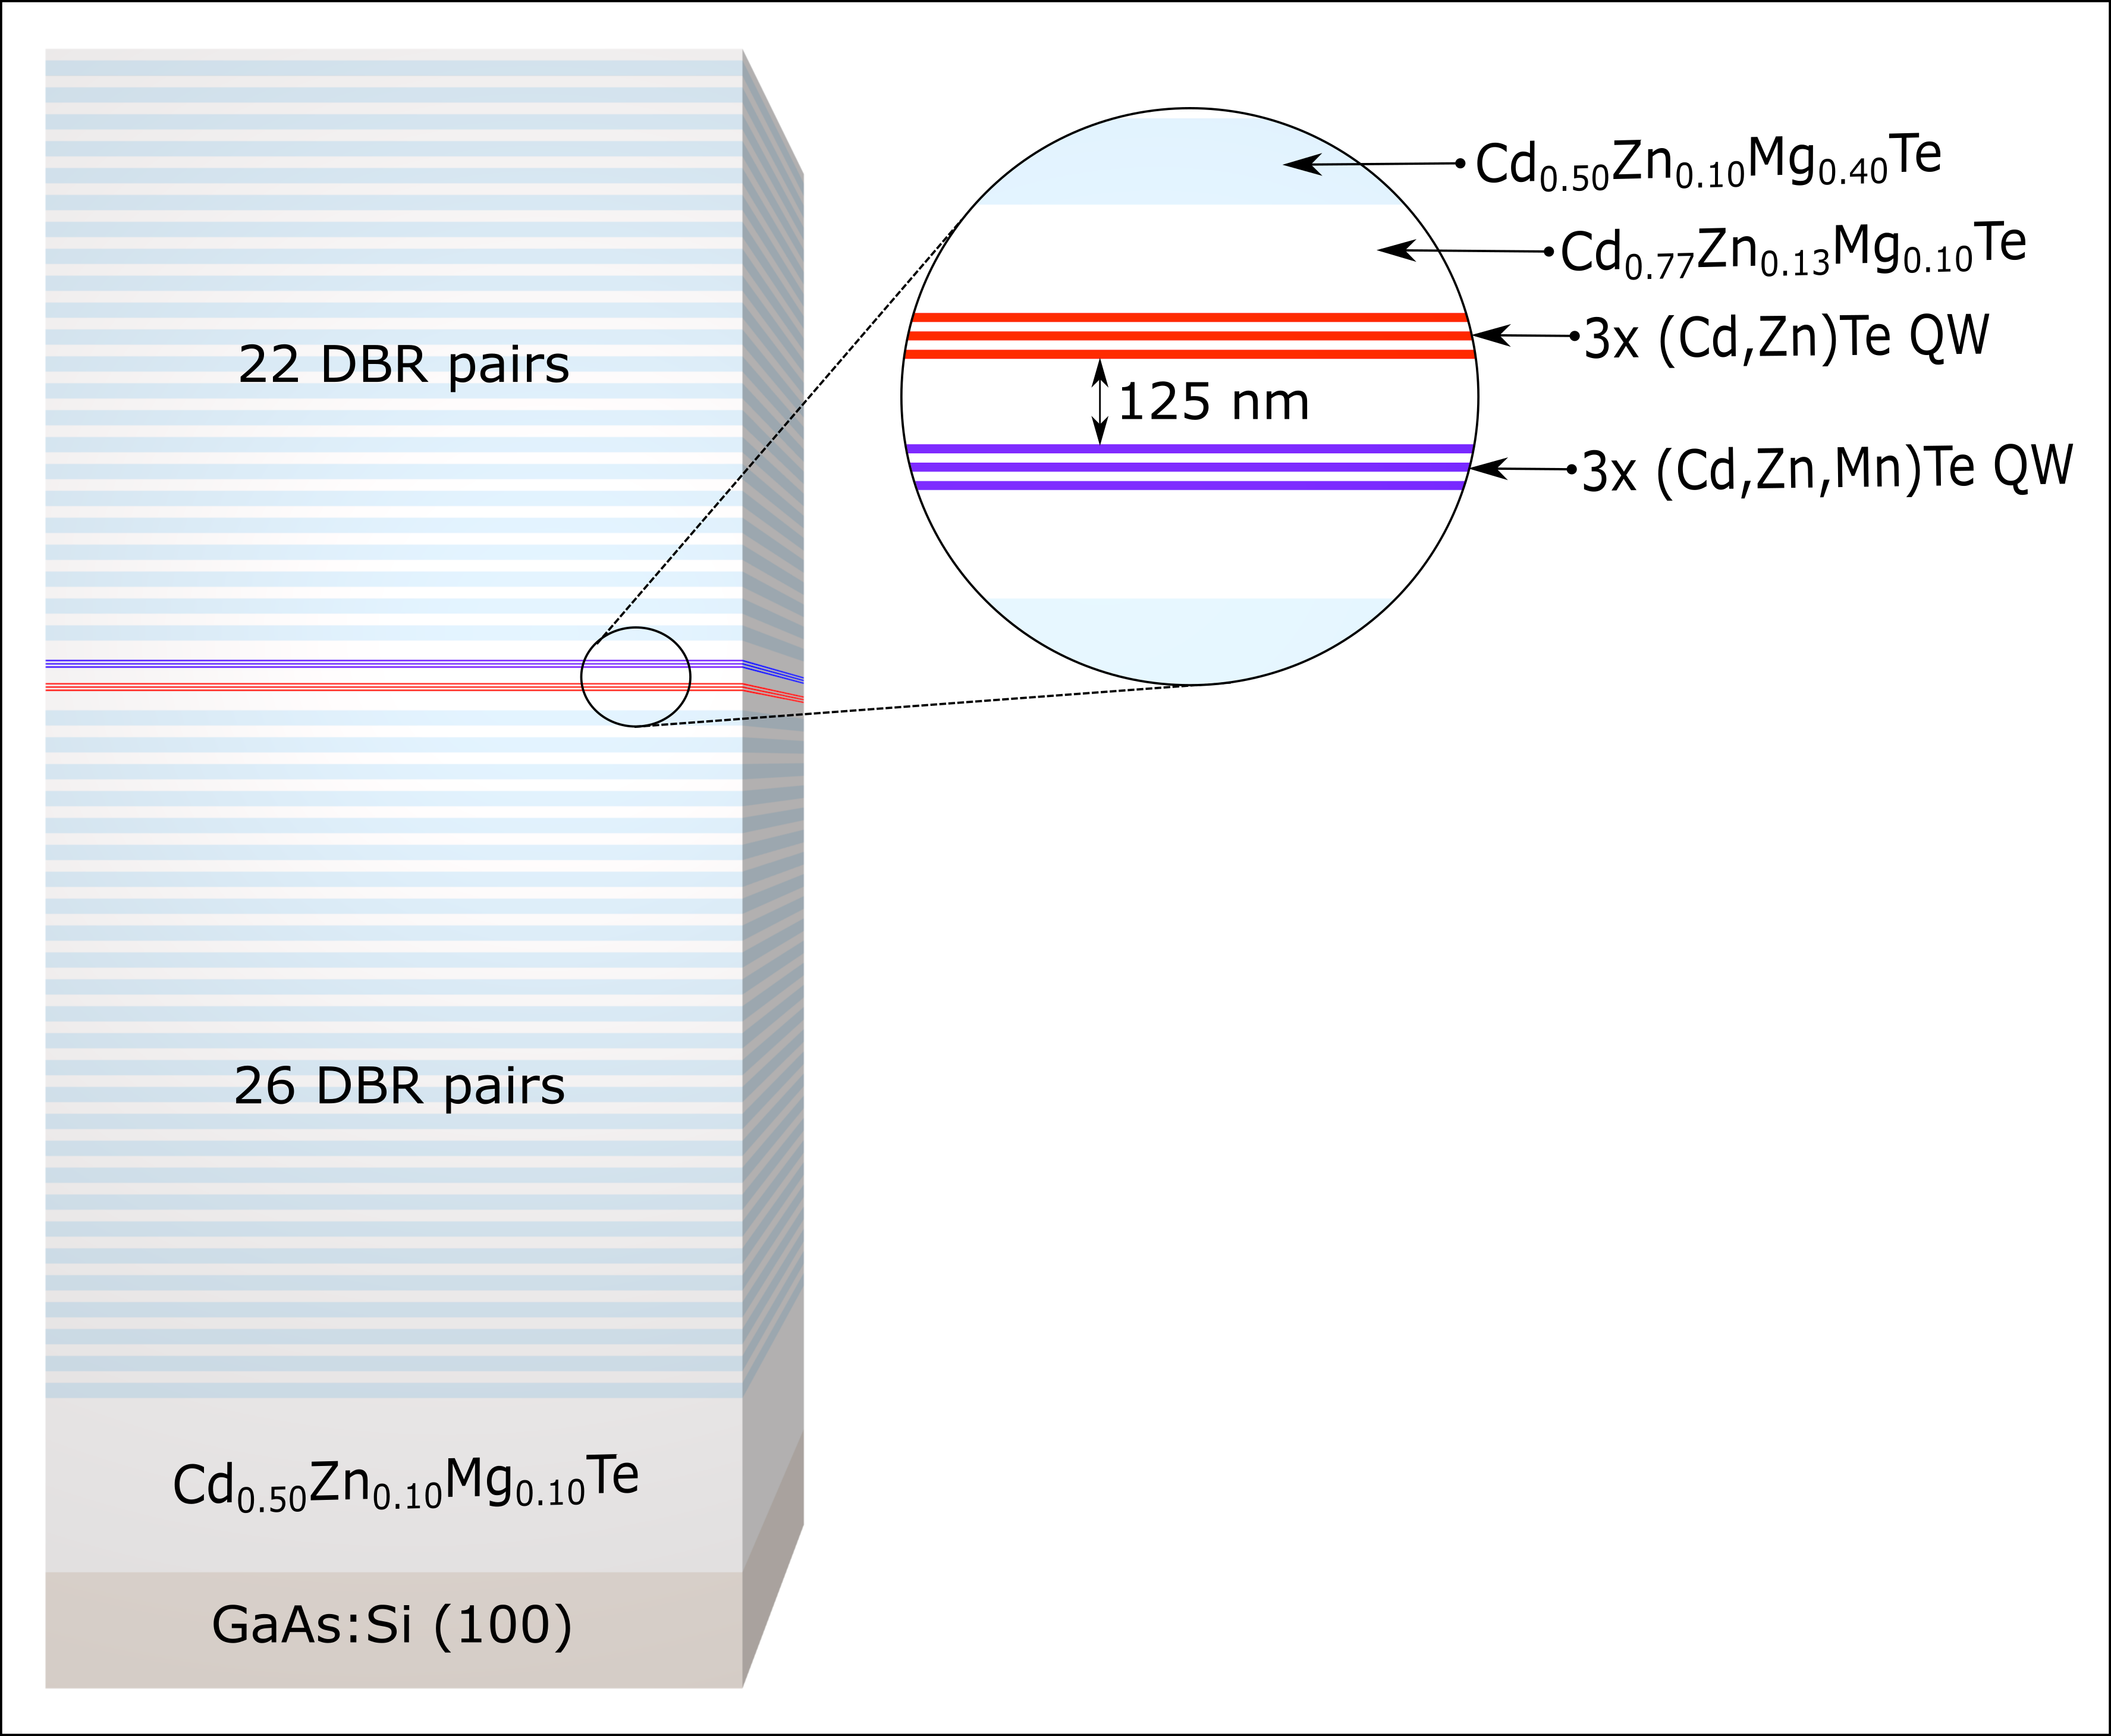
\includegraphics[width=13cm]{Probka} 
\centering
\caption{Schemat próbki.}
\end{figure}

Studnie tu wykorzystane są wykonane z materiału typu DMS, czyli półprzewodnika półmagnetycznego. Materiał tego typu wykazuje właściwości zarówno półprzewodnikowe jak i magnetyczne, pozwalając np. na kontrolę jego poziomów energetycznych przy pomocy pola magnetycznego.

\chapter{Metody eksperymentalne}\label{r:metody}
Do wzbudzania ekscytonów wykorzystano laser od długości fali 685 nm, 


\chapter{Wyniki}\label{r:wyniki}
\section{Wyniki surowe}
\section{Dopasowanie do modelu}




\chapter{Podsumowanie}


\appendix

\chapter{Może będzie potrzebne}

\bibliographystyle{plain}
\bibliography{bibliografia}

\end{document}


%%% Local Variables:
%%% mode: latex
%%% TeX-master: t
%%% coding: latin-2
%%% End:
